\subsection{Концепция изолобальной аналогии с позиции метода молекулярных орбиталей. Изолобальные ряды}

Изолобальная аналогия - одинаковое число граничных орбиталей(высших занятых и низших валентных) со сходными свойствами, близкими энергиями и одинаковым числом электронов.

\begin{figure}[H]
\centering
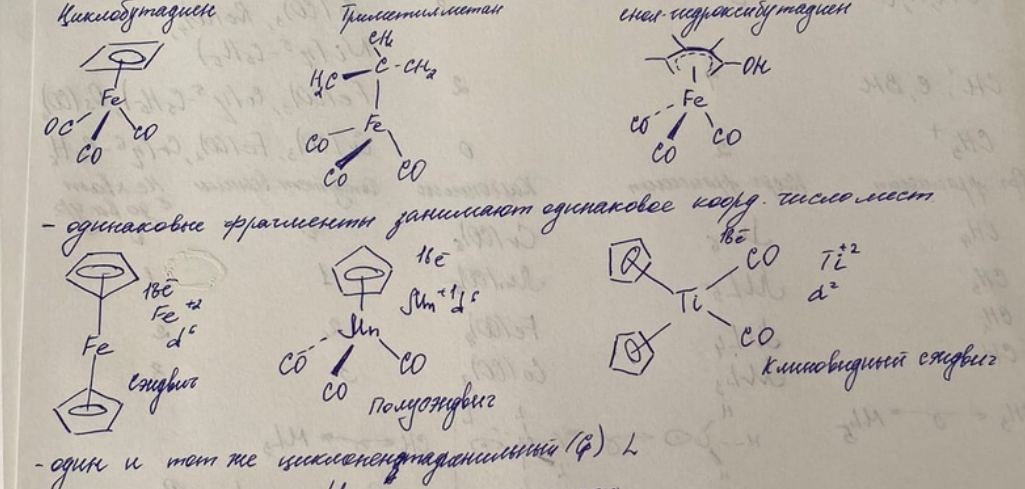
\includegraphics[scale=.300]{images/isolab_examples.png}
\end{figure}

\subsubsection*{Электроноэквивалентные}
\begin{tabular}{|l|l|l|}
\hline
	Недостающие электроны & Гл. группа & Карбонилы\\
\hline
	1 & Cl,Br,I(7e) & $Mn(CO)5$, $Co(CO)_4$ - 17e\\
\hline
	2 & S(6e) & $Fe(CO)_4$, $Os(CO)_4$ - 16e\\
\hline
	3 & P(5e) & $Co(CO)_3$, $Ir(CO)_3$ - 15e\\
\hline
\end{tabular}



\begin{tabular}{|l|l|l|l|l|l|}
\hline
1 & \multicolumn{5}{l|}{К.ч. металла на котором построена аналогия} \\ \hline
Орг. фрагмент & 9    & 8   & 7   & 6 & 5   \\ \hline
$CH_3$ & $d^1ML_8$   & $d^3ML_7$   & $d^5ML_6$   & $d^7ML_5$ & $d^9ML_4$  \\ \hline
$CH_2$ & $d^2ML_7$    & $d^4ML_6$   & $d^6ML_5$   & $d^*ML_4$ & $d^10ML_3$   \\ \hline
$CH$ & $d^3ML_6$    & $d^5ML_5$   & $d^7ML_4$   & $d^9ML_3$ & NA   \\ \hline
\end{tabular}


\subsection*{Изолабпльные соотношения}


\begin{tabular}{|l|l|l|l|}
\hline
\multicolumn{1}{|l|}{Орг.группа} & \multicolumn{1}{l|}{валент. e} & \multicolumn{1}{l|}{скелетные e} & \multicolumn{1}{l|}{металлооорганические примеры} \\ \hline
\multicolumn{1}{|l|}{$CH_3$}     & \multicolumn{1}{l|}{7}         & \multicolumn{1}{l|}{5}           & \multicolumn{1}{l|}{$Mn(CO)_5, Fe(CO)_5,Mo(CO)_3(\eta^5-C_5H_5)$}                             \\ \hline
\multicolumn{1}{|l|}{$CH_3^+$}   & \multicolumn{1}{l|}{6}         & \multicolumn{1}{l|}{4}           & \multicolumn{1}{l|}{$Cr(CO)_5,PtCl_3^-,, Mn(CO)_2(\eta^5-C_5H_5)$}                             \\ \hline
\multicolumn{1}{|l|}{$CH_2$}     & \multicolumn{1}{l|}{6}         & \multicolumn{1}{l|}{4}           & \multicolumn{1}{l|}{$Fe(CO)_4, Cr(CO)_5, Cu(\eta^5-C_5H_5)$}                             \\ \hline
$CH, N, O^+$                     & 5                              & 3                                &       $Co(CO)_3, Re(CO)_4, Ni(\eta^5-C_5H_5) $                                            \\ \hline

$CH^+, C, BH$                    & 4                              & 2                                & $Fe(CO)_3, OS(CO)_3$                              \\ \hline

$CH_3^+$                         & 2                              & 3                                & $Cr(CO)_3, Fe(CO)_2, Cr(\eta^6PhH)$                  \\ \hline

                                              
\end{tabular}

И еще немного

\begin{tabular}{|l|l|l|l|l|}
\hline
Орг. фрагмент & Неорг. фрагмент & Карбонил   & Отсутст. вершин & Не хват. электронов \\ \hline
$CH_4$        & $ML_6$          & $Cr(CO)_6$ & 0               & 0                   \\ \hline
$CH_3$        & $ML_5$          & $Mn(CO)_5$ & 1               & 1                   \\ \hline
$CH_2$        & $ML_4$          & $Fe(CO)_4$ & 2               & 2                   \\ \hline
$CH$          & $ML_3$          & $CO(CO)_3$ & 3               & 3                   \\ \hline
\end{tabular}

\begin{figure}[H]
\centering
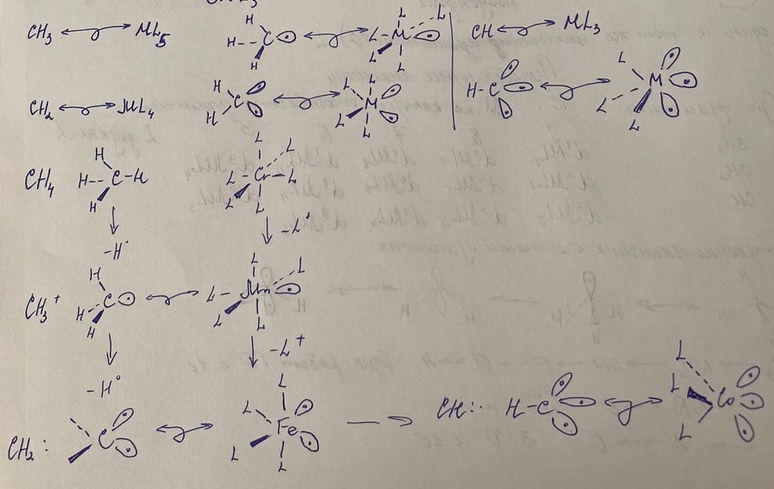
\includegraphics[scale=.300]{images/isolab_2.png}
\end{figure}


\begin{figure}[H]
\centering
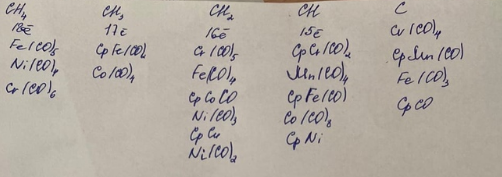
\includegraphics[scale=.300]{images/isolab_3.png}
\end{figure}







